%%%%%%%%%%%%%%%%%%%%%%%%%%%%%%%%%%%%%%%%%
% Beamer Presentation
% LaTeX Template
% Version 1.0 (10/11/12)
%
% This template has been downloaded from:
% http://www.LaTeXTemplates.com
%
% License:
% CC BY-NC-SA 3.0 (http://creativecommons.org/licenses/by-nc-sa/3.0/)
%
%%%%%%%%%%%%%%%%%%%%%%%%%%%%%%%%%%%%%%%%%

%----------------------------------------------------------------------------------------
%	PACKAGES AND THEMES
%----------------------------------------------------------------------------------------

\documentclass{beamer}

\mode<presentation> {

% The Beamer class comes with a number of default slide themes
% which change the colors and layouts of slides. Below this is a list
% of all the themes, uncomment each in turn to see what they look like.

%\usetheme{default}
%\usetheme{AnnArbor}
%\usetheme{Antibes}
%\usetheme{Bergen}
%\usetheme{Berkeley}
%\usetheme{Berlin}
%\usetheme{Boadilla}
%\usetheme{CambridgeUS}
%\usetheme{Copenhagen}
%\usetheme{Darmstadt}
% \usetheme{Dresden}
%\usetheme{Frankfurt}
%\usetheme{Goettingen}
%\usetheme{Hannover}
%\usetheme{Ilmenau}
%\usetheme{JuanLesPins}
%\usetheme{Luebeck}
\usetheme{Madrid}
%\usetheme{Malmoe}
%\usetheme{Marburg}
%\usetheme{Montpellier}
%\usetheme{PaloAlto}
%\usetheme{Pittsburgh}
%\usetheme{Rochester}
%\usetheme{Singapore}
%\usetheme{Szeged}
%\usetheme{Warsaw}

% As well as themes, the Beamer class has a number of color themes
% for any slide theme. Uncomment each of these in turn to see how it
% changes the colors of your current slide theme.

% \usecolortheme{albatross}
% \usecolortheme{beaver}
%\usecolortheme{beetle}
%\usecolortheme{crane}
%\usecolortheme{dolphin}
% \usecolortheme{dove}
%\usecolortheme{fly}
%\usecolortheme{lily}
%\usecolortheme{orchid}
%\usecolortheme{rose}
%\usecolortheme{seagull}
%\usecolortheme{seahorse}
%\usecolortheme{whale}
%\usecolortheme{wolverine}

%\setbeamertemplate{footline} % To remove the footer line in all slides uncomment this line
\setbeamertemplate{footline}[page number] % To replace the footer line in all slides with a simple slide count uncomment this line

\setbeamertemplate{navigation symbols}{} % To remove the navigation symbols from the bottom of all slides uncomment this line
}

\usepackage{graphicx} % Allows including images
\usepackage{booktabs} % Allows the use of \toprule, \midrule and \bottomrule in tables
%\usepackage {tikz}
\usepackage{physics}
\usepackage{mathtools}
\usepackage{tkz-graph}
\usepackage[round]{natbib}
\GraphInit[vstyle = Shade]
\tikzset{
  LabelStyle/.style = { rectangle, rounded corners, draw,
                        minimum width = 2em, fill = yellow!50,
                        text = red, font = \bfseries },
  VertexStyle/.append style = { inner sep=5pt,
                                font = \normalsize\bfseries},
  EdgeStyle/.append style = {->, bend left} }
\usetikzlibrary {positioning}
%\usepackage {xcolor}
\definecolor {processblue}{cmyk}{0.96,0,0,0}
%----------------------------------------------------------------------------------------
%	TITLE PAGE
%----------------------------------------------------------------------------------------

\title[Short title]{AI Based Lecture Summarization Tool} % The short title appears at the bottom of every slide, the full title is only on the title page

\author{
  Team 9\\
} % Your name
\institute[IIIT-H] % Your institution as it will appear on the bottom of every slide, may be shorthand to save space
{
IIIT Hyderabad\\ % Your institution for the title page
\medskip
}
\date{\today} % Date, can be changed to a custom date

\begin{document}

\begin{frame}
\titlepage % Print the title page as the first slide
\end{frame}

\begin{frame}
\frametitle{Overview} % Table of contents slide, comment this block out to remove it
\tableofcontents % Throughout your presentation, if you choose to use \section{} and \subsection{} commands, these will automatically be printed on this slide as an overview of your presentation
\end{frame}

%----------------------------------------------------------------------------------------
%	PRESENTATION SLIDES
%----------------------------------------------------------------------------------------

%------------------------------------------------
\section{Problem Statement}
\begin{frame}{Problem Statement}
Despite the many advantages of online learning, it faces some severe disadvantages such as:
    \begin{itemize}
        \item Lack of accessibility due to internet connectivity issues
        \item Low attention span of students as compared to physical learning in classroom settings
        \item Uploaded videos are difficult to revise as compared to class notes
    \end{itemize}
\end{frame}

\begin{frame}{Problem Statement}
As part of our end semester project in Software Engineering, we aim to address a few of
the above problems by using AI to automatically summarize lecture videos. Our solution would
leverage the latest advancements in machine learning and computer vision to make it very easy for users to revise using the uploaded videos. 
\end{frame}

\section{Our Solution}
\begin{frame}{Our Solution}
    We have developed our software using a client-server architecture and the user interacts with our product using a web application.
    \begin{itemize}
        \item The client side provide the user with a UI where they are able to login, and add, search and summarize the videos
        \item The server deal with all the client side requests such as:
            \begin{itemize}
                \item Provide authentication methods for login
                \item Summarize a given uploaded video
                \item Return the most relevant clips for a given search query
            \end{itemize}
        \item Our solution uses a combination of video processing, machine learning and summarization techniques to solve the problem in a fast and efficient manner. 
    \end{itemize}
\end{frame}

\section{High Level Design of our algorithm}
\begin{frame}{High Level Design}
\begin{figure}
    \centering
    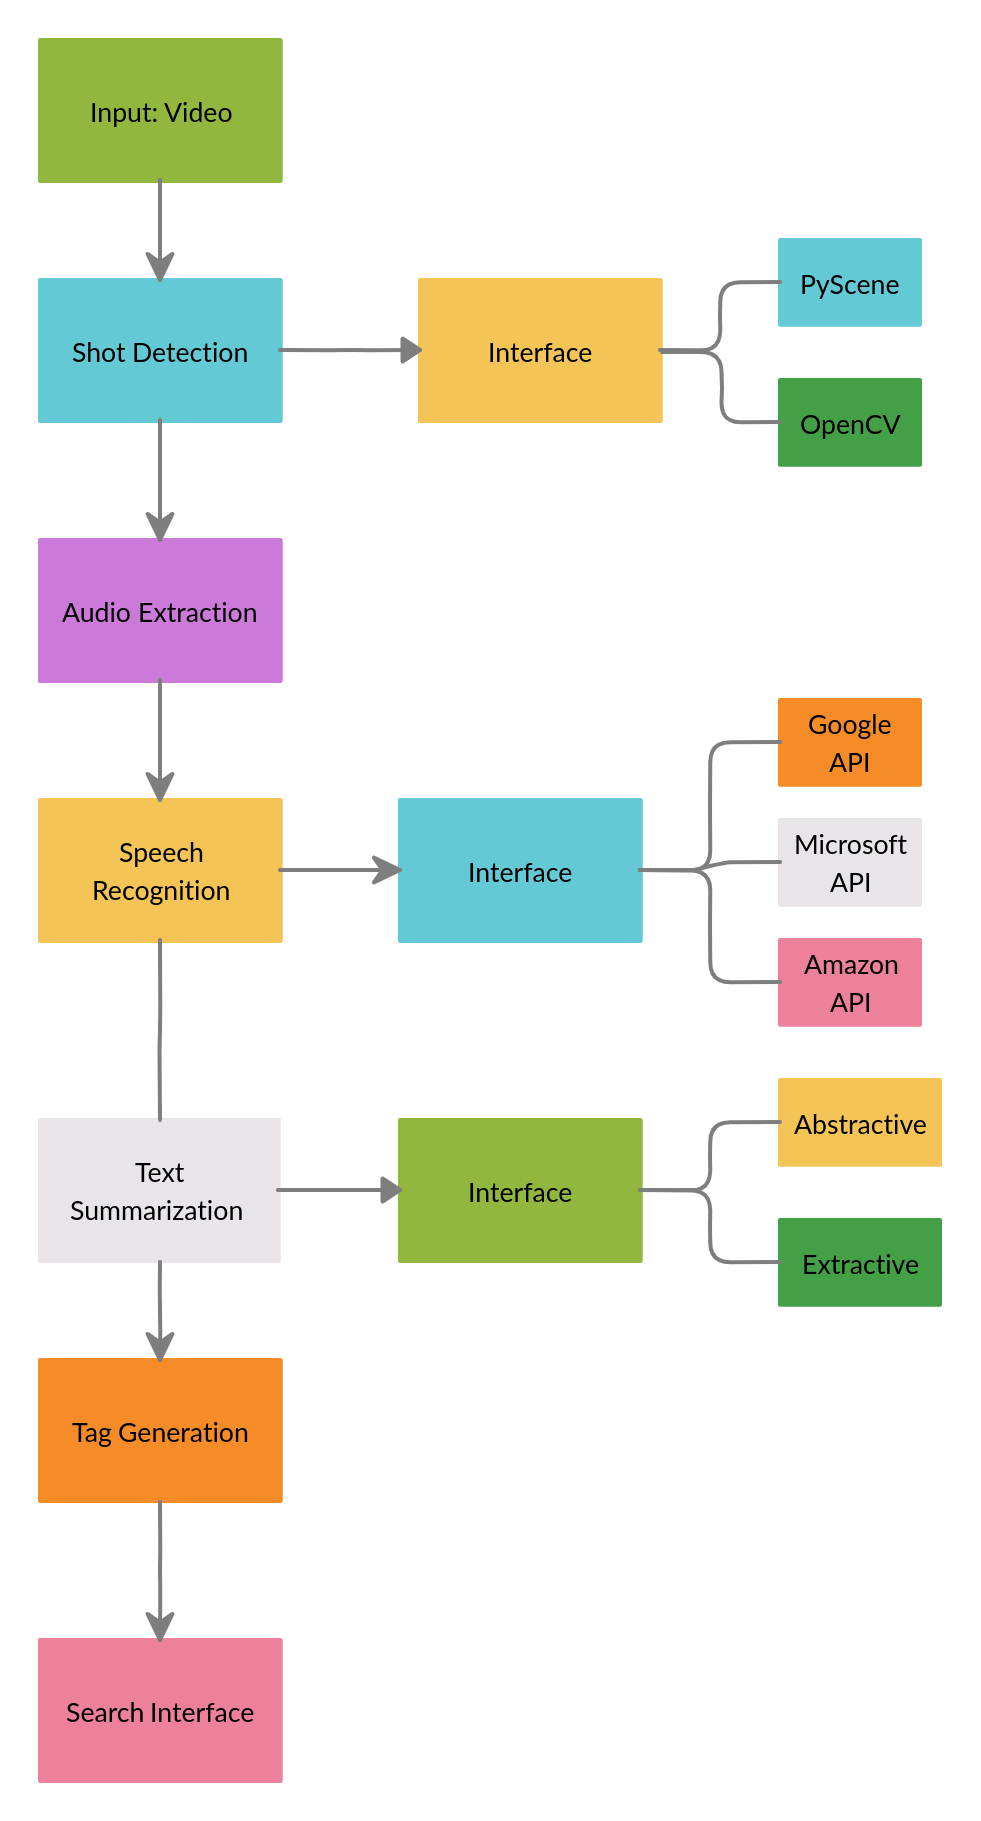
\includegraphics[scale=0.11]{Block Level Diagram.png}
    \caption{High Level Design of our algorithm}
    \label{fig:HLD}
\end{figure}
\end{frame}

\section{Coding Principles and Design Patterns}
\begin{frame}{Coding Principles and Design Patterns}
    \begin{itemize}
        \item We have followed Model View Template \textbf{Design Patterns}. The Model is the logical data structure behind the entire application and is represented by a database. The View is the user interface and template consists of static parts of the HTML output as well as describes how dynamic content will be inserted. 

        \item Follows object oriented paradigm, which is a sub category of imperative programming paradigm. 

        \item Interfaces and objects are created for each of the sub modules.
        \item Functions names are self-explanatory and small in size (7-10) lines.
        \item Exceptions are handled by using try except blocks.
        \item The code of different sub modules is easily \textbf{extendable} to other APIs and libraries.
        \item Followed \textbf{SOLID} design principles.
    \end{itemize}
\end{frame}

\section{Software Development Model}
\begin{frame}{Software Development Model}
    \begin{itemize}
        \item Agile SDLC Model
        \item Feature Driven Development (FDD) Agile methodologies 
        \item Great solution to maintain control for incremental Agile project management 
    \end{itemize}
\end{frame}

\section{Integration and Testing}
\begin{frame}{Integration and Testing Process}
    \begin{itemize}
        \item Unit Testing
            \begin{itemize}
                \item Each module has its test files in its respective folder. 
            \end{itemize}
        \item After Unit Testing we have performed \textbf{Incremental Integration Testing}.
            \begin{itemize}
                \item Integrate the modules one by one using stubs or drivers to uncover the defects.
                \item We have used \textbf{Functional} incremental testing methodologies as integration and testing takes place on the basis of the functionalities as per the requirement specifications in design document.
            \end{itemize}
        \item We have used this because the defects are found early in a smaller assembly when it is relatively easy to detect the root cause of the same.
    \end{itemize}
\end{frame}


% \begin{frame}{References}
% % \bibliographystyle{acm}
% \bibliographystyle{unsrt}
% \bibliography{references}
% \end{frame}

% \begin{frame}
% \begin{figure}
%     \includegraphics[scale=0.3]{withthanks.jpg}
% \end{figure}
% \end{frame}

\end{document}

